\section[Itération~1:~(~2/22/2017~-~3/5/2017~)]{Itération~1:~\textup{\textto{(~2/22/2017~-~3/5/2017~)}}}

\subsection{Introduction}

La méthodologie Scrum consiste à développer le produit incrémentalement, en
effet chaque itération résulte un prototype ayant des fonctionnalité du produit
demandé livrable. Le développement de ces fonctionnalité est en parallèle avec
d'autre fonctionnalité puisque l'équipe avance dans le même niveaux.

\subsection{Objectif de l'itération}

L'objectif de cette itération vise deux environnement:

\begin{description}
    \item [Mobile] Créer une première version d'application mobile permettant
        de localiser des utilisateurs selon leur position actuelle.
    \item [Web] Projeter instantanément la position de l'utilisateur sur une
        carte map avec son état (activé ou désactivé)
\end{description}

\begin{figure}[htbp]
    \centering
    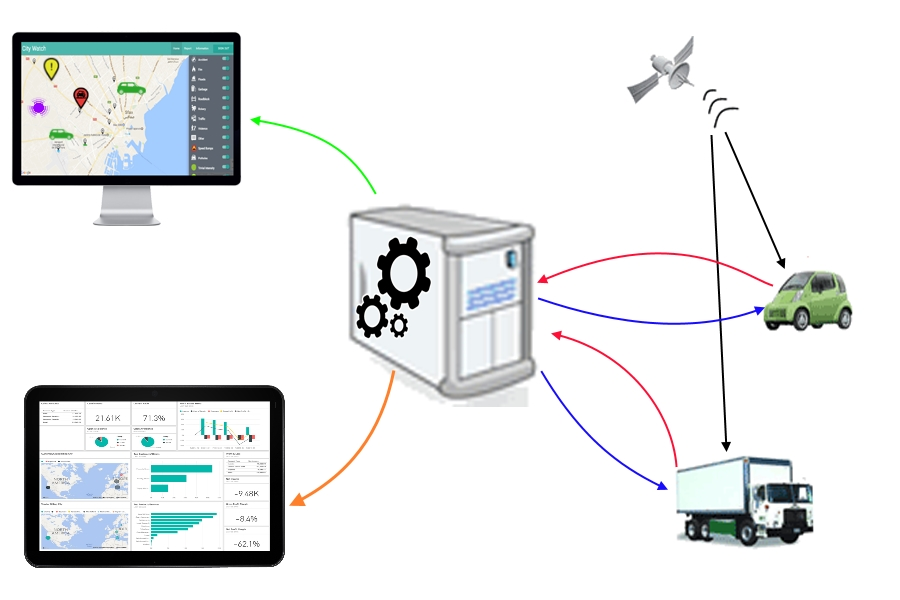
\includegraphics[width=0.8\textwidth]{citywatch-architecture}
    \caption[Flux des information Géographiques en CityWatch]
    {Flux des informations Géographiques dans le système de localisation}
    \captionsource{}{http://masterhaniff.blogspot.com/2014/11/vehicle-tracking-system.html}
    \label{fig:citywatch-architecture}
\end{figure}

%L'objectif de cette itération est d'étudier notre Serveur, de générer notre
%modèle, de réaliser la page Web (dashboard) et développer les vues nécessaires
%pour permettre à l'utilisateur de consulter la dernière position du véhicule
%selon les spécifications du Backlog.

%Une fois la première ébauche du Backlog est réalisée, le Product Owner peut
%découper les spécifications de haut niveau vers des spécifications plus
%raffinées. Dès lors, nous passons à la planification d'une itération. Il est
%important de rappeler que les premières spécifications du Backlog doivent être:

%\begin{itemize}
%    \item assez précise pour être estimée par l'équipe.
%    \item assez petite pour être développée et testée durant une itération.
%\end{itemize}

%Ayant une bonne idée sur le produit ainsi que l'objectif à atteindre, l'équipe
%et le Product Owner peuvent passer à l'élaboration des itérations. Dans notre
%projet \textquote{Plateforme CityWatch}, la durée d'une itération est fixée à
%trois semaines. Dans cette section, nous décrivons le déroulement de la
%première itération. Une itération commence par sa planification et finit par
%être revue avec le \textquote{Product Owner}.

\subsection{Planification de l'itération}

Dans le but de définir le périmètre fonctionnel de l'itération 1 et faire sa
planification, tous les membres de l'équipe ont participé à un réunion avec le
Scrum Master et le Product Owner pour définir le backlog du sprint.

La planification de l'itération représente une étape importante dans la vie de
l'itération parce que au cours du planification, on divise l'itération a
plusieurs tâches pour mieux atteindre le résultats attendu à la fin de
l'itération.

Dans cette première itération, on a décidé de diviser cette itération en trois
grandes parties:

\begin{enumerate}
    \item Une partie consacrée pour la création de la base de donnée et les
        services web.
    \item Une partie consacré pour la réalisation de la page d'accueil.
    \item Une partie qui répond aux besoins des autres tâches de cette
        itérations.
\end{enumerate}

\subsubsection{Backlog de l'Itération}

Les tâches à réaliser peuvent \HTODO{être soient}{contenir?} des tâches de
recherche, de documentation, de conception, de développement ou bien
d'installation, de tests, d'intégration, etc\ldots. Il est recommandé lors de
la planification de la liste des tâches de bien les détailler. Une tâche ne
doit pas inclure d'autres tâches. Ceci permet de bien cerner le travail
demandé.

\begin{center}
    \footnotesize
    \begin{longtable}{| p{1cm} | p{5cm} | p{7cm} | p{1cm} |}
        \caption{Backlog de l'itération 1}
        \label{tab:sprint1-backlog} \\

        \hline
        \textbf{Réf} & \textbf{Spécification} & \textbf{Description} & \textbf{Priorité} \\ \hline
        \endhead

        \hline \multicolumn{4}{|r|}{{Continué en page suivante$\dotsc$}} \\ \hline
        \endfoot

        \hline \hline
        \endlastfoot

        \hline
1.1 & Présentation et Configuration SVN & Présenter SVN, installer le serveur SVN et créer les répertoires & 1 \\ \hline
1.2 & Recherche sur les Services Web & Présenter les différentes Solutions des services web et choisir la meilleur solution & 1 \\ \hline
1.3 & Implémenter service Save Position & Enregistrement les coordonnées requis dans la base de données & 2 \\ \hline
1.4 & Implémenter la consommation du service Save Position & Coordonnées enregistrés instantané et continuellement dans la BD & 1 \\ \hline
1.5 & Recherche sur les spécifications de la plateforme Android & Présenter le modèle de développement Android et choisir le SDK optimale & 1 \\ \hline
1.6 & Création squelette de l'application mobile & Application fonctionnel (sans les fonctions de localisation) avec l'IHM nécessaire et l'intégration au SVN & 1 \\ \hline
1.7 & Implémenter service Get Last Position & Le serveur retourne les dernières coordonnées requis & 1 \\ \hline
1.8 & Rectification service Save Positon & Support multiple périphériques et enregistrer la date d'envoyé & 2 \\ \hline
1.9 & Rectification service Get Last Position & Retourné la position du périphérique et la date du dernier modification & 2 \\ \hline
1.10 & Affiche Multiple marqueurs & Afficher dernière position de chaque périphérique dans la carte & 2 \\ \hline
1.11 & Affiche état du périphérique & Afficher si le périphérique est en ligne ou hors ligne & 3 \\ \hline
    \end{longtable}
\end{center}

\subsubsection{Estimation de la Première Itération}

Nous avons fixé la période d'une itération à 3 semaine. Dans le
tableau~\ref{tab:sprint1-capacity}, nous présentons une estimation du nombre
d'heures pendant lesquelles nous nous engageons à travailler.

\begin{table}[htbp]
    \centering
    \begin{tabular}{| c | c | c | c |}
        \hline
        \textbf{Membre} & \textbf{Nombre d'heures par jour} & \textbf{Nombre de jours présent} & \textbf{Total en heures} \\ \hline
        \hline

Moez & 6 & 10 & 60\\ \hline
Rihab & 6 & 10 & 60 \\ \hline
\multicolumn{2}{c|}{} & \textbf{Total} & 120 \\ \cline{3-4}
    \end{tabular}
    \caption{Nombre d'heures de travail estimé de l'itération 1}
    \label{tab:sprint1-capacity}
\end{table}

Tout les membres de l'équipe font ensuite l'estimation de temps (en point
d'histoire d'utilisateur) de chaque tache avec le poker de planning. Les
estimmations utilisés sont $\frac{1}{2}$, $1$, $2$, $3$, $5$, $8$, $13$. Les
taches peuvent aussi étre assignées aux plus qu'un seul membres.

Le tableau~\ref{tab:sprint1-estimation} représente les éstimations de nos
taches en heures (x2 signifie que la tache était assigné à deux membres) et le
membre à qui étati assigné la tache.

\begin{center}
    \begin{longtable}{| l | l | l |}
        \caption{Nombre d'heures estimé pour la réalisation des taches}
        \label{tab:sprint1-estimation} \\

        \hline
        \textbf{Spécification} & \textbf{Membre} & \textbf{Heures} \\ \hline
        \endhead

        \hline \multicolumn{3}{|r|}{{Continué en page suivante$\dotsc$}} \\ \hline
        \endfoot

        \hline \hline
        \endlastfoot

        \hline
Présentation et Configuration SVN & Rihab & 5 x 2 \\ \hline
Recherche sur les Services Web & Moez & 13 x 2 \\ \hline
Implémenter service Save Position & Moez & 5 \\ \hline
Implémenter la consommation du service Save Position & Rihab & 5 x 2 \\ \hline
Recherche sur les spécifications de la plateforme Android & Rihab & 13 x 2 \\ \hline
Création squelette de l'application mobile & Rihab & 13 \\ \hline
Implémenter service Get Last Position & Moez & 5 \\ \hline
Rectification service Save Positon & Moez & 5 \\ \hline
Rectification service Get Last Position & Moez & 5 \\ \hline
Affiche Multiple marqueurs & Moez & 5 \\ \hline
Affiche état du périphérique & Rihab & 5 \\ \hline
    \end{longtable}
\end{center}

\subsubsection{Évolution du travail}

Au cours de l'itération, on a utilisé Excel et un tableau physique pour suivre
l'évolution des taches de chaque membre.

\clearpage % FIXME

Dans les figures~\ref{fig:sprint1-fig1},~\ref{fig:sprint1-fig2}
et~\ref{fig:sprint1-fig2}, on représente l'état du tableau des taches en jour
de distribution les taches, au milieu et à la fin de l'itération
respectivement. Les lignes colorés représentent nos taches. Les colonnes du
tableau sont:

\begin{description}
    \item [Who] L'allias du nom de chaque membres de l'équipe .

            \emph{Exemple }: RM signifie \textbf{R}ihab \textbf{M}ajdoub
    \item [À faire (Todo)] Les taches assignés au membres pour cette itération.
        L'échange des taches entre les membres est possible sur le supervision
        du Scrum Master.
    \item [Implémentation] La pourcentage de l'implémentation du tache de 0\%
        jusqu'à 100\%. Si le développeur a commencé l'implémentation d'une
        tache, il la déplace dans cette colonne et faire le mise à jour du
        pourcentage de l'implémentation à chaque jour pendant un court réunion
        nommée \textquote{Daily Scrum} pendant le, on discute l'évolution du
        travail et le plan du jour prochain.
    \item [Test/Intégration/Review] L'implémentation du tache est complete,
        elle est donc en phase d'évaluation et vérification de son
        fonctionnement si intégré dans le reste du système. Depuis la deuxième
        itération, au moins un autre membre doit revue le code pour à fin
        d'assurer la qualité du code, détecter et corriger les défauts le plus
        tôt possible.
    \item [Complete (Done)] La tache était implémentée et validée.
\end{description}

On a utilisé des différents couleurs pour différents types des taches:

\begin{description}
    \item [Rose] Les taches du développement d'interface web (Dashboard).
    \item [Verte] Les taches du développement mobile (l'application Android).
    \item [Jaune] Les taches du développement des services web et d'administration.
\end{description}

La liste des prochaines réunions est écrite dans le tableau aussi:

\begin{itemize}
    \item Présentations des recherches si la taches inclue une partie du
        recherche et présentation.
    \item Rendez-Vous avec des autres personnes concernés par le projet.
    \item Si un développeur est besoin d'aide ou de discusser un probleme
        recontré.
    \item Code Revue à la fin d'itération fait par tous les membres pour
        évaluer la qualité du code et détecter les défaults du conception et
        d'implementation.
\end{itemize}

\begin{figure}[htbp]
    \centering
    \caption{Évolution du travail}
    \begin{subfigure}{1\textwidth}
        \centering
        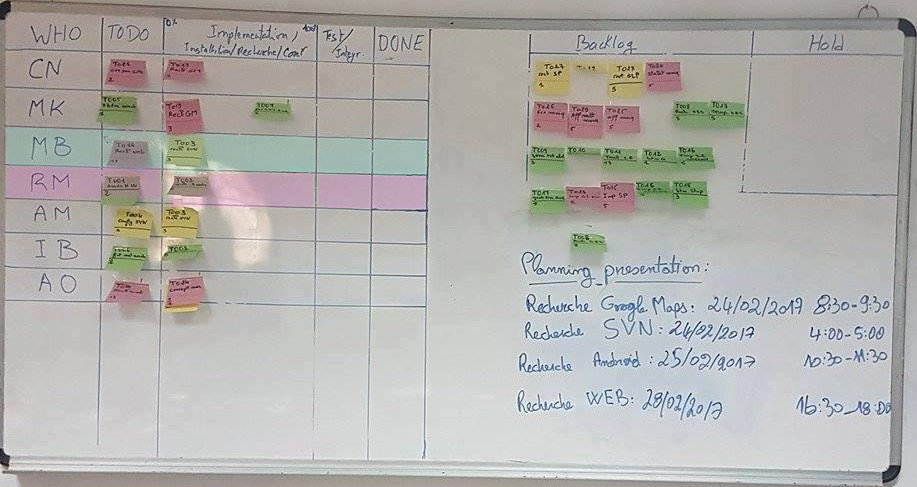
\includegraphics[width=0.8\textwidth]{sprint1-fig1}
        \caption{Distribution des taches de l'itération}
        \label{fig:sprint1-fig1}
    \end{subfigure}

    \begin{subfigure}{1\textwidth}
        \centering
        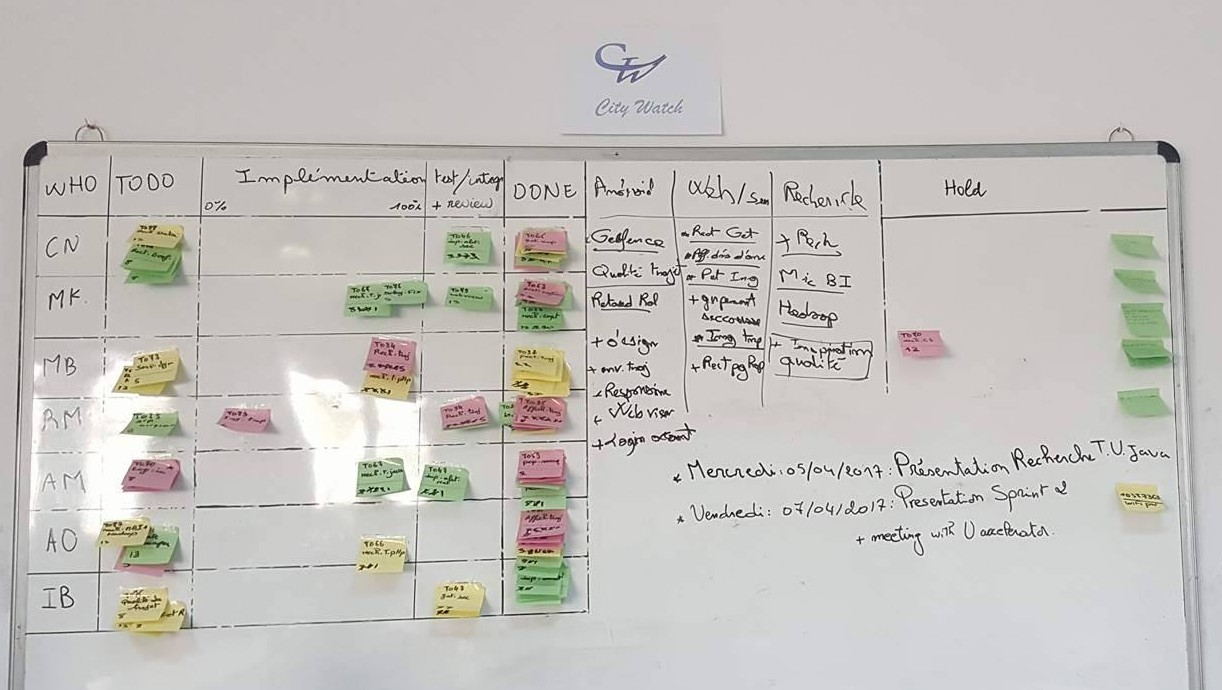
\includegraphics[width=0.8\textwidth]{sprint1-fig2}
        \caption{Au milieu d'itération}
        \label{fig:sprint1-fig2}
    \end{subfigure}

    \begin{subfigure}{1\textwidth}
        \centering
        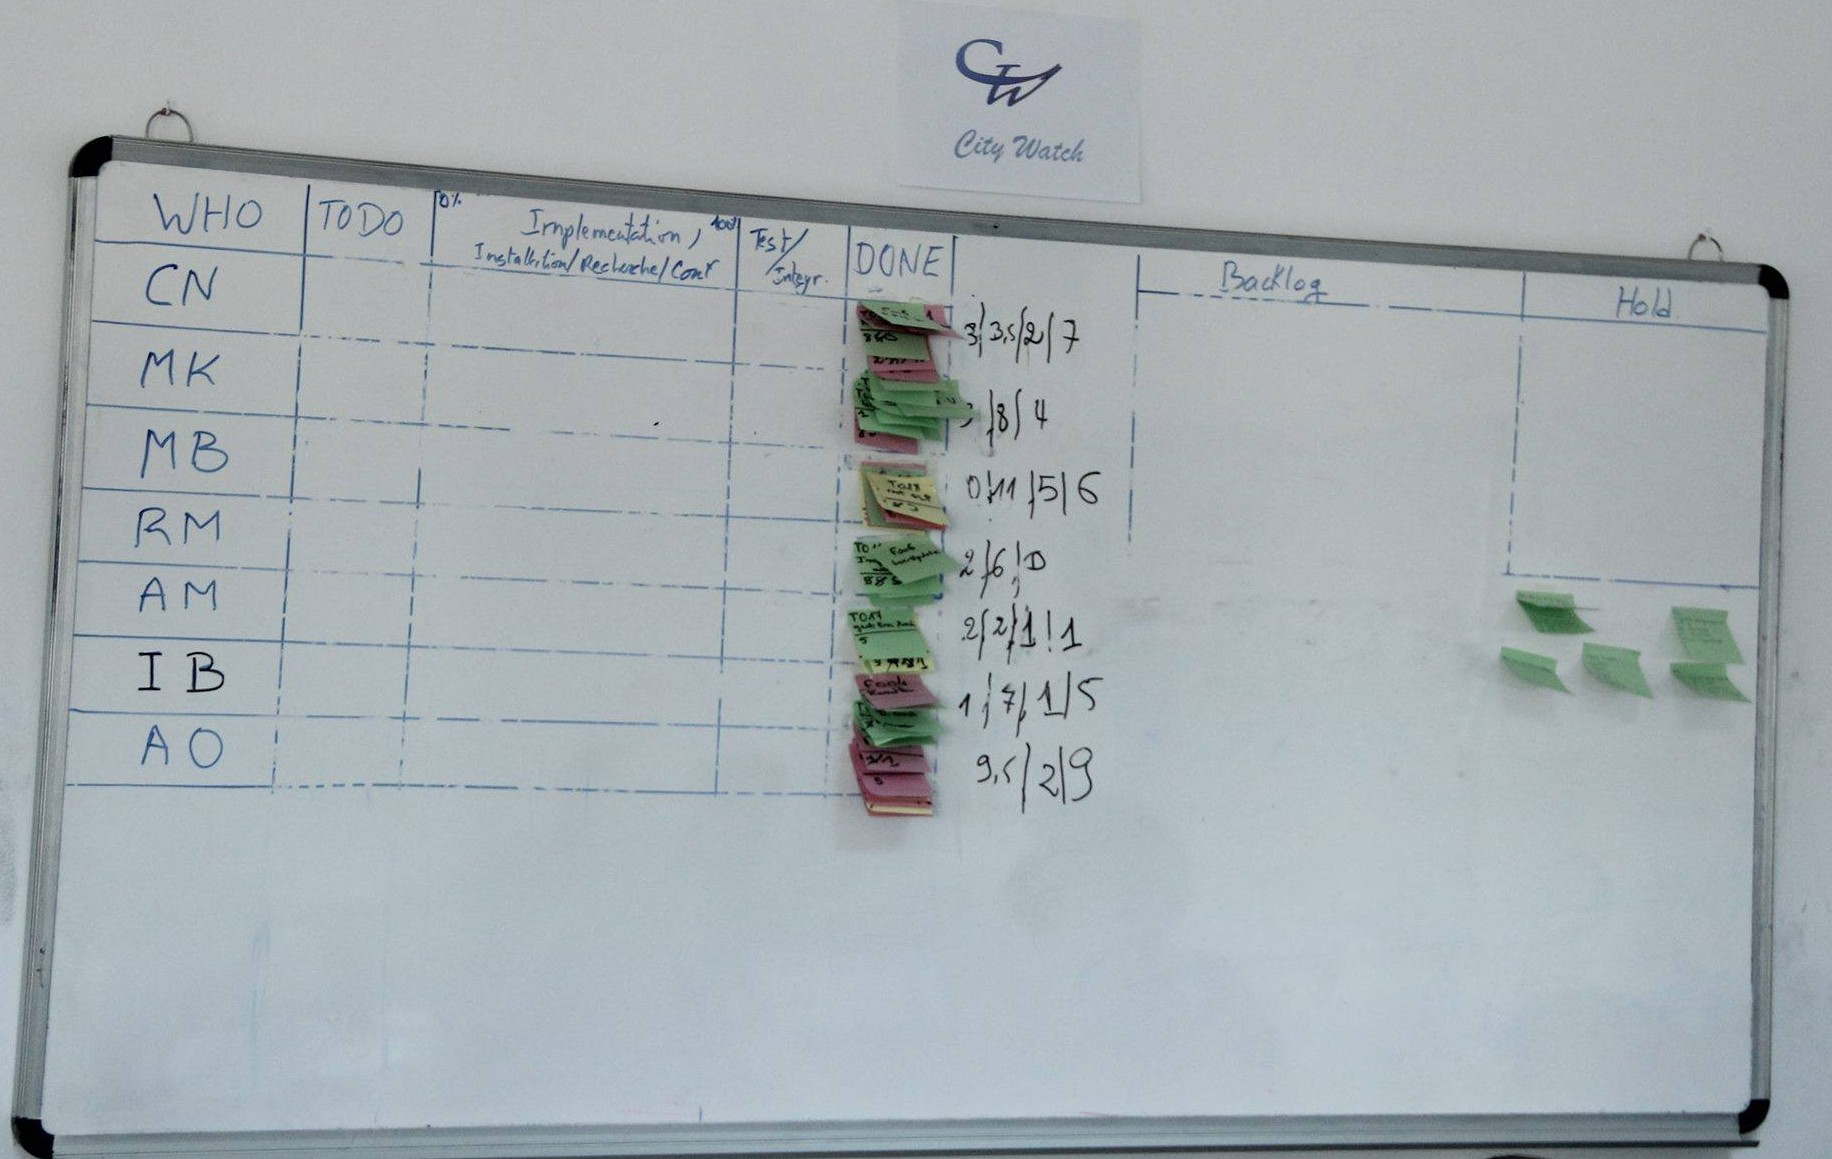
\includegraphics[width=0.8\textwidth]{sprint1-fig3}
        \caption{Au fin d'itération}
        \label{fig:sprint1-fig3}
    \end{subfigure}
\end{figure}
\clearpage

\subsection{Présentation des outils utilisés}

Le stage chez Djagora Academy nous a permis d'acquérir de nouvelles compétences
tant au niveau relationnel que technique. Pour bien entamer la réalisation de
la plateforme \textquote{City Watch}, nous avons suivi différentes formations
sur les outils et les technologies que nous venons de citer.

\subsubsection{Apache Subversion}

Les logiciels de gestion de versions \acrshort{VCS} nous permettent de
conserver la chronologie des modifications du source de code, ainsi récupérer
les version intermédiaires et les différences entre eux, et facilitent la
collaboration au développement. Les deux logiciels de gestion de versions les
plus répondus sont Git et Apache SVN\@.

\begin{description}
    \item [Git] Logiciel de gestion de versions distribué avec des branches
        légères. La récupération des versions précédentes et l'enregistrement
        des changements sont possibles sans besoin d'accès au dépôt distant car
        chaque développeur a une copie complète du dépôt. Le modèle Fork
        (Dupliquer), Commit (Modifier), Merge (Fusionner) a eu un grand succès
        dans les projets libres.
    \item [Apache SVN] Logiciel de gestion de versions centralisé. Il est connu
        pour sa simplicité comme il n'est pas un distinct entre un dépôt local
        vs. Dépôt distant, on faire juste une copie du dossier de travail d'une
        version précise. Les commandes sont simples:
        \begin{itemize}
            \item \verb|svn checkin| \ \ vs. \ \ \verb|git commit; git push|
            \item \verb|svn update| \ \ vs. \ \ \verb|git fetch; git rebase|
        \end{itemize}
        Le support du Windows est excellent surtout les outils graphiques. La
        plus tard des fonctionnalités du SVN nécessitent l'accès au dépôt
        (distant).
\end{description}

Apache SVN était choisi pour sa simplicité, sa bon support de Windows et pour
des exigences de spécification. \FIXME{improve sentence}

L'outil serveur choisi est VisualSVN Server pour sa simplicité d'installer et
de configurer et pour son support du Windows.

Les outils clients choisis sont:

\begin{itemize}
    \item TortoiseSVN pour l'intégration avec le système Windows.
    \item La commande de ligne \verb|svn| est utilisée en Linux.
    \item Le support de SVN est intégré au Android Studio et PHPStorm.
\end{itemize}

%Un logiciel de gestion de versions est un logiciel de gestion de configuration
%permettant de stocker des informations pour une ou plusieurs ressources
%informatiques permettant de récupérer toutes les versions intermédiaires des
%ressources, vainsi que les différences entre les versions.
%
%Apache Subversion (en abrégé SVN) est un logiciel de gestion de versions,
%distribué sous licence Apache et BSD\@.
%VisualSVN est un plug-in d'intégration de Subversion de qualité professionnelle.
%Les principaux avantages de VisualSVN sont les suivants:
%
%\begin{itemize}
%    \item Fiabilité imbattable: Visual Studio ne s'arrêtera jamais ni ne
%        s'arrêtera à cause de VisualSVN.
%    \item Intégration transparente: VisualSVN gère automatiquement les fichiers
%        ajoutés ou renommés et reflète ces opérations sur Subversion.
%    \item Statut en temps réel: VisualSVN suit attentivement et affiche toutes
%        les modifications apportées à votre copie de travail.
%    \item Courbe d'apprentissage courte: VisualSVN utilise les boîtes de
%        dialogue TortoiseSVN et fournit un assistant intelligent pour mettre
%        vos sources sous Subversion.
%\end{itemize}
%VisualSVN Server vous permet d'installer et de gérer facilement un serveur
%Subversion entièrement fonctionnel sur la plateforme Windows. Il est utile tant
%pour les petites entreprises que pour les entreprises.

\subsubsection{Android}

Android est un système d'exploitation conçu en 2007 \TODO{référence} par la
société Android, startup racheté par Google. Android est Open Source, ça veut
dire on peut lire le code de ce logiciel le modifier et le redistribuer.

\paragraph{Activity:}

Un utilisateur habile d'Android remarque que lors de l'exploitation d'une
application Android qu'il est en train de naviguer entre des fenêtres et
l'application ne afficher qu'une seule fenêtre à la fois ces fenêtre la sont
des activités on peut différencier ces activité a travers leur interface
graphique ceci s'applique sur la plupart des application Android car il y a des
applications qui contiennent pas d'activités. Un première idée qui nous frappe
la tète c'est que une activité est un conteneur d'élément graphique qui
constitue un interface graphique. Alors que ne non une activité n'est pas
seulement une interface graphique mais elle va établir les liens entre
l'interface graphique et la logique programma tique de plus l'activité contient
des informations sur le statut actuel de l'application qui s'appelle le
contexte ce contexte permet de faire la liaison entre le système Android et les
autres activités de l'application.

\subparagraph{États d'activités:}

Le système Android met en place un système priorités entre application par
exemple l'utilisateur est en train de naviguer sur internet et écouter de la
musique il reçois un appel comme l'application qui gère les appel est une
application plus prioritaire elle prend la du navigateur et le lecteur musique
pour que l'utilisateur puisse répondre a son appel. Si une application consomme
trop de ressources et peut bloquer le fonctionnement du système Android,
Android arrêtera cette application. Et aussi comme expliqué précédemment les
activités sont gères a partir d'un système de pile d'activités. D'où
l'apparition de plus d'un état qui sont centré sur l'activité.

On peut différencier ces états par leur visibilité:

\begin{itemize}
    \item État Active.
    \item État en Pause.
    \item État Arrêté.
\end{itemize}

\subparagraph{Cycle de vie d'une activité:}

Une activité n'a pas de contrôle sur son état. Son état change suivant un cycle
rythmique entre le système Android et les autres application (un système quasi
dépendant sur des priorités comme expliqué précédemment). La
figure~\ref{fig:android-activity} explique le cycle de vie d'une activité. Les
états sont représentés comme des méthodes parce que lors de la programmation,
ces états sont interroges par le nom de ces méthodes.

% Diagram of Android activity life cycle
% Author: Pavel Seda 
% Drawing part, node distance is 1.5 cm and every node
% is prefilled with white background
\begin{figure}[H]
 \centering
 \footnotesize

\begin{tikzpicture}[node distance=1.5cm,
    every node/.style={fill=white, font=\sffamily}, align=center]
  % Specification of nodes (position, etc.)
  \node (start)             [activityStarts]              {L'activité démarre};
  \node (onCreateBlock)     [process, below of=start]          {onCreate()};
  \node (onStartBlock)      [process, below of=onCreateBlock]   {onStart()};
  \node (onResumeBlock)     [process, below of=onStartBlock]   {onResume()};
  \node (activityRuns)      [activityRuns, below of=onResumeBlock]
                                                      {Activity is running};
  \node (onPauseBlock)      [process, below of=activityRuns, yshift=-1cm]
                                                                {onPause()};
  \node (onStopBlock)       [process, below of=onPauseBlock, yshift=-1cm]
                                                                 {onStop()};
  \node (onDestroyBlock)    [process, below of=onStopBlock, yshift=-1cm] 
                                                              {onDestroy()};
  \node (onRestartBlock)    [process, right of=onStartBlock, xshift=4cm]
                                                              {onRestart()};
  \node (ActivityEnds)      [startstop, left of=activityRuns, xshift=-4cm]
                                                        {Le processus est tué};
  \node (ActivityDestroyed) [startstop, below of=onDestroyBlock]
                                                    {l'activité est arrêtée};     
  % Specification of lines between nodes specified above
  % with aditional nodes for description 
  \draw[->]             (start) -- (onCreateBlock);
  \draw[->]     (onCreateBlock) -- (onStartBlock);
  \draw[->]      (onStartBlock) -- (onResumeBlock);
  \draw[->]     (onResumeBlock) -- (activityRuns);
  \draw[->]      (activityRuns) -- node[text width=4cm]
                                   {Une autre activité s'intercole devent notre activité} (onPauseBlock);
  \draw[->]      (onPauseBlock) -- node {Notre activité n'est plus visible}
                                   (onStopBlock);
  \draw[->]       (onStopBlock) -- node {L'activité est arrêtée par le système ou l'utilisateur} (onDestroyBlock);
  \draw[->]    (onRestartBlock) -- (onStartBlock);
  \draw[->]       (onStopBlock) -| node[yshift=1.25cm, text width=3cm]
                                   {L'activité revientsur le devant de la scène}
                                   (onRestartBlock);
  \draw[->]    (onDestroyBlock) -- (ActivityDestroyed);
  \draw[->]      (onPauseBlock) -| node(priorityXMemory)
                                   {Priorité élevée $\rightarrow$ plus mémoire}
                                   (ActivityEnds);
  \draw           (onStopBlock) -| (priorityXMemory);
  \draw[->]     (ActivityEnds)  |- node [yshift=-2cm, text width=3.1cm]
                                    {L'utilisateur retourne vers l'activité}
                                    (onCreateBlock);
  \draw[->] (onPauseBlock.east) -- ++(2.6,0) -- ++(0,2) -- ++(0,2) --
     node[xshift=1.2cm,yshift=-1.5cm, text width=2.5cm]
     {L'activité revient sur le devant de la scéne}(onResumeBlock.east);

  \end{tikzpicture}
  \caption{Diagramme de cycle de vie d'activite Android}
  \captionsource{Pavel Seda, \TeX example.net [Modifié]}{http://www.texample.net/tikz/examples/android/}
  \label{fig:android-activity}
\end{figure}


\subparagraph{Comment choisir le SDK optimale:}

Une SDK permet l'application de marcher sur la version Android visé et les
versions ultérieure il a noté de prendre en considération le taux des
utilisateurs visé par cette application. Aussi il faut travailler avec une SDK
digne de confidence qui n'a pas de problème ou bug qui peuvent bloquer ou
arrêter le fonctionnement de l'application le SDK choisi doit pouvoir supporter
les fonctionnalité offerte par l'application si on va utiliser une
fonctionnalité qui utilise les empreinte le SDK dont on a travailler
l'application doit supporter cette fonctionnalité lorsque le travail sur une
application est en groupe il est mieux que tous ce groupe utilise la même SDK
pour éviter tous problème de compatibilité et conflit entre versions de SDK
donc il faut choisir une SDK qui est populaire en utilisation et qui est
stable. Dans notre projet on va utiliser SDK 23 qui vise la version Android 6.0
ayant un taux d'utilisateur qui est 4.79 % des utilisateur d'Android notons que
cet SDK comporte la fonctionnalité d'Android les plus récentes et qui est
stable.

\subsubsection{Les Services Web}

Un service web est un protocole d'interface de communication et l'échange de
données entre applications et systèmes hétérogènes à distance en utilisant les
technologies Web (HTTP dans notre cas).

Pendant la conception de l'api du service de position, on a étudié les
différentes variantes des architectures des services web:

\begin{itemize}
    \item Orienté RPC (ex: XML-RPC, SOAP, JSON-RPC):
        \begin{itemize}
            \item Meilleur pour présenter des actions et commandes.
        \end{itemize}
    \item Orienté Ressources (ex: RESTful):
        \begin{itemize}
            \item Représenter les données sous formes des ressources.
            \item Utiliser les méthodes HTTP pour modifier/créer/lire/supprimer
                les données.
            \item Utiliser les paramètres d'URL pour passer des paramètres.
            \item Sans état.
            \item Meilleur pour modéliser un domaine et entités.
        \end{itemize}
\end{itemize}

On a choisi d'utiliser l'architecture RESTful comme notre API est mieux décri
comme ensemble des collections des données dont on peut effectuer avec des
actions CRUD\@.

\subsection{Mises des normes}

Les exigence de l'api RESTful sont:

\begin{description}
    \item [Performance] Le temps de réponse doit être en une durée raisonnable.
    \item [Multi-Utilisateurs] On doit avoir la possibilité de stocker et
        récupérer les positions des différents utilisateurs.
    \item [Stabilité] L'implémentation doit vérifier la structure des données
        reçus, la disponibilité des champs obligatoires et leurs formats.
    \item [Portabilité] Le système doit support la différence en zone du temps
        et en internalisation, format de présentation des données géologique et
        sa précision.
\end{description}


\subsection{Conception}

\begin{figure}[htbp]
    \centering
    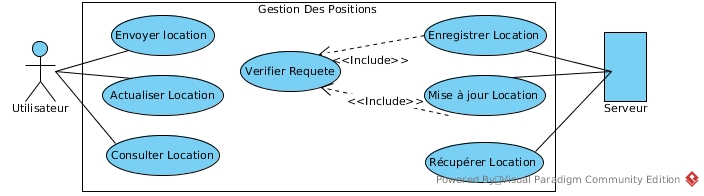
\includegraphics[width=1\textwidth]{sprint1-webservices-usecase}
    \caption{Diagramme de case d'utilisation du services web en itération 1}
    \label{fig:sprint1-webservices-usecase}
\end{figure}

%\begin{figure}[htbp]
%    \centering
%    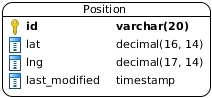
\includegraphics[width=0.45\textwidth]{sprint1-webservices-database}
%    \caption{Diagramme entité-association du service Position en itération 1}
%\end{figure}

\begin{figure}[htbp]
    \centering
    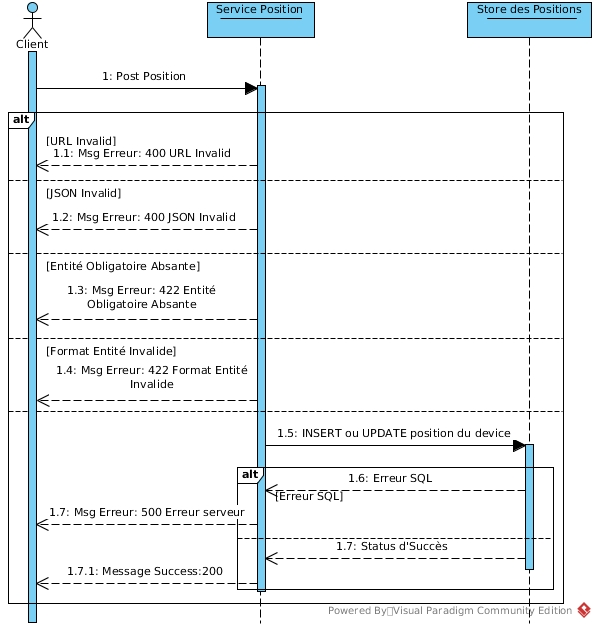
\includegraphics[width=1\textwidth]{sprint1-webservices-post-sequence}
    \caption{Diagramme de séquence du service Post Position en itération 1}
    \label{fig:sprint1-webservices-post-sequence}
\end{figure}

\begin{figure}[htbp]
    \centering
    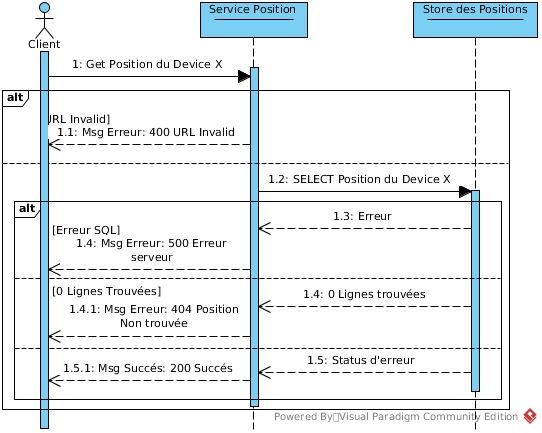
\includegraphics[width=1\textwidth]{sprint1-webservices-get-sequence}
    \caption{Diagramme de séquence du service Get Position en itération 1}
    \label{fig:sprint1-webservices-get-sequence}
\end{figure}

\subsection{Évaluation suivant les normes mise}

Avant de commencer le développement, on a fixé quelques règles à respecter pour
assurer la qualité du code.

\begin{itemize}
    \item Activer le mode strict du PHP et changer le mode de traitement des
        erreurs au déclenchement des exceptions si possible (PDO, \ldots).
        Activer le mode strict du JavaScript aussi.
    \item Utiliser des analyseurs statiques du code: PHP\_CodeSniffer, PHPLint
        et ESLint pour détecter les erreurs formelles de programmation ou de
        conception.
    \item Documenter chaque fonction, classe, constante et variable global. On
        a utilisé PHPDoc, apiDoc et JSDoc pour documenter le code PHP, l'api
        RESTful et le code JavaScript respectivement.
    \item Ecrire les tests unitaires pour les fonctions et les classes selon la
        technique \acrshort{TDD}. On a autorisé l'ecrire des tests unitaires
        aprés le développement du code. Les outils utilisés sont PHPUnit pour
        PHP et Mocha/Chai pour JavaScript. \TODO{Move to sp2}
\end{itemize}

Dans 1\ier{} phase, on a implémenté les méthodes POST et GET du ressource
Position. L'architecture résultante est documentée dans
l'annexe~\ref{appendix:sprint1-position-post-doc}
et~\ref{appendix:sprint1-position-get-doc}.

On a essayé d'adresser les différents les mises des normes spécifiés;

\subsubsection{Performance}

On a minimisé la dépendance en bibliothèques externes et extensions PHP\@. De
plus, Le nombre des requêtes SQL ont étés minimisés à une seule requêtes pour
chaque méthode du notre service web.

\subsubsection{Multi-Utilisateurs}

Les positions à enregistrer doivent contenus un id qui doit être utilisé aussi
pour retirer la dernière position. On a utilisé diffèrent identificateur pour
chaque périphériques basé sur le MAC du phone.

\subsubsection{Portabilité}

On a utilisé la format standardisée JSON~\cite{ECMA-404} pour le transfert de
données ce qui assure la portabilité des représentations des différents types
des données (nombres, booléens, strings, \ldots) indépendant du
l'internationalisation (séparateur décimal, \verb|true| vs. \verb|True| vs.
\verb|vrai| vs. \verb|yes| vs. \verb|y|, \ldots).

Pour le représentation des dates dans le content du requêtes HTTP, on a utilisé
la format RFC3339~\cite{RFC3339} (basé sur ISO8601~\cite{ISO8601} pour
l'utilisation dans les protocols du Web) avec UTC comme la défaut zone du
temps, ex: \verb|2005-08-15T15:52:01Z|.

Pour les en-têtes du requêtes HTTP, la format de représentation des dates est
RFC1123~\cite{RFC1123}, ex: \verb|Mon, 15 Aug 2005 15:52:01 +0000|.

La format du présentation des positions géologique (latitude et longitude)
choisie est la même représentation des nombres en JSON avec une précision
jusqu'à 14 chiffres après le séparateur décimal. Les valeurs envoyés doivent
respecte l'intervalle des diffèrent entités géologiques ($latitude \in [-90,
90]$, $longitude \in [-180, 180]$)

\subsubsection{Stabilité}

Pour assuré la stabilité d'un service web, on doit vérifier la validité de
contenu reçu même si envoyé depuis un source de confiance avant de les
utiliser. La vérification inclue le test de disponibilité des entités
obligatoires et le test de leurs formats.

\TODO{tips from Heroku HTTP API design guide}

\subsection{Contributions}

On avait des problèmes pour le chargement du code à notre serveur causés par le
blockage du port FTP et inefficacité de compresser le code et le charger depuis
l'interface web chaque fois. On a décidé d'automatiser ce tache avec un script.
Après inspecter et étudier l'api d'interface web du serveur FTP, on a
implémenté un script Python qui compresse les fichiers nécessaires, authentifie
au service web du serveur FTP et charger l'archive.

\subsection{Revue de cette itération}

À la fin de l'itération, notre équipe et le \textquote{Product Owner} invitées
se réunissent pour effectuer la revue de sprint, qui dure au maximum quatre
heures.

L'objectif de la revue de l'itération est de valider l'incrément de produit qui
a été réalisé pendant cette itération. L'équipe énonce les éléments du backlog
en début de sprint, et présente les taches finis\footnote{complètement
réalisés}.

Une fois le bilan du sprint réalisé, l'équipe de développement et le
\textquote{Product Owner} mettent à jour le carnet du produit en fonction de ce
qui a été réalisé (fini).

\subsubsection{Produit de l'itération}

A la fin de l'itération 1, nous avons un première produit partiel permettant de
suivre la position des multiple smartphones et les afficher dans la carte de
notre site web.

\paragraph{Page Web \textquote{Dashboard}}

La figure~\ref{fig:sprint1-dashboard-screenshot} affiche la position des
individus et son état.

\begin{itemize}
    \item \textit{Marqueur en Vert}: Périphérique en ligne.
    \item \textit{Marqueur en Rouge}:Périphérique en hors ligne.
\end{itemize}

\begin{figure}[htbp]
    \centering
    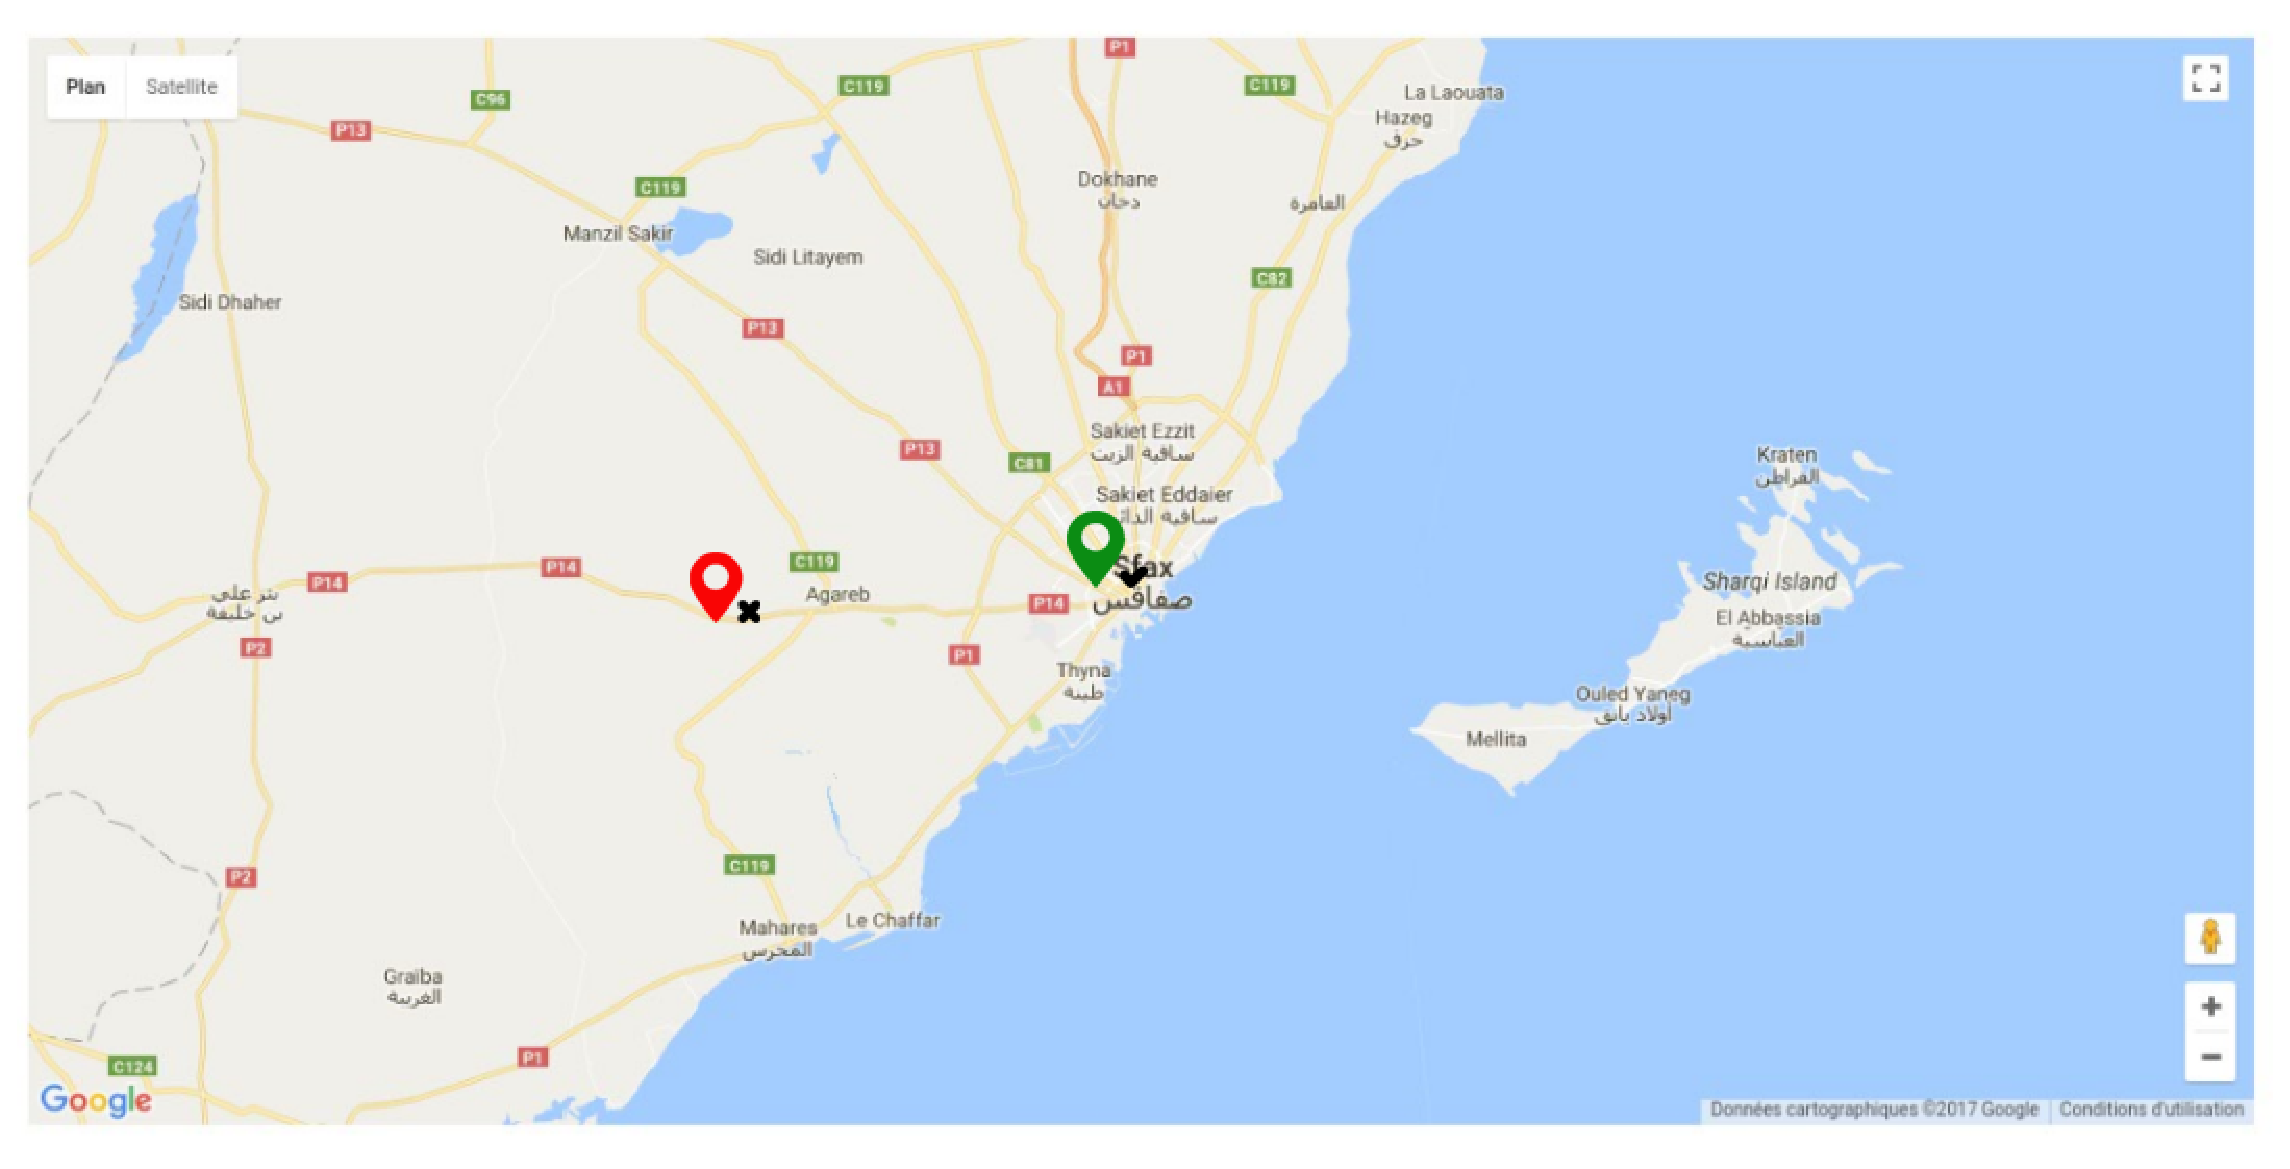
\includegraphics[width=0.6\textwidth]{sprint1-dashboard-screenshot}
    \caption{Capture écran de la page web de l'itération 1}
    \label{fig:sprint1-dashboard-screenshot}
\end{figure}

\paragraph{Application Android}

La figure~\ref{fig:sprint1-android-screenshot} représente l'interface de
l'application.

\begin{figure}[htbp]
    \centering
    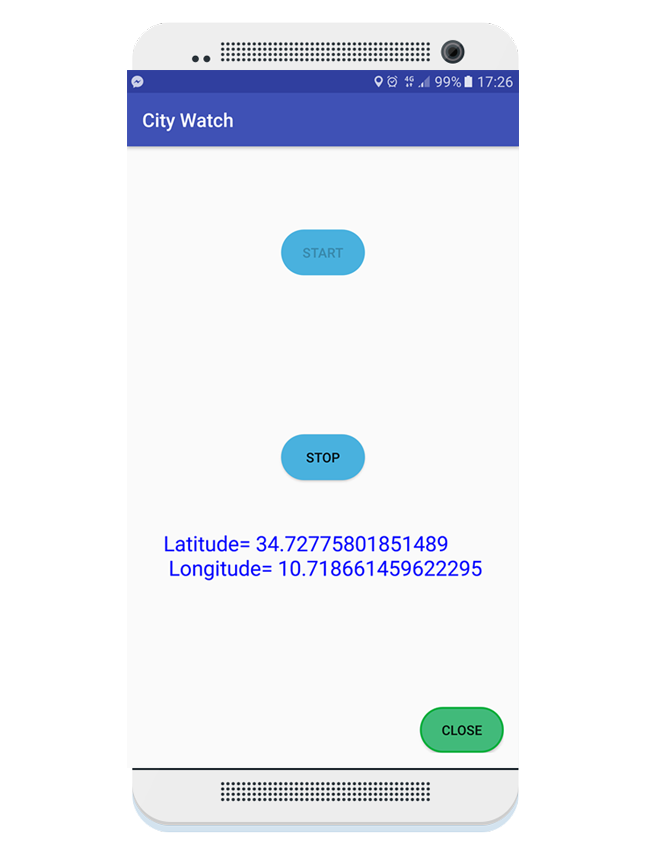
\includegraphics[width=0.45\textwidth]{sprint1-android-screenshot}
    \caption{Capture écran d'application Android de l'itération 1}
    \label{fig:sprint1-android-screenshot}
\end{figure}

\subsubsection{Avis du Product Owner}

Le Product Owner était ravi des résultats de cette première itération. Il a
validé donc notre travail et nous a encouragé pour l'élaboration des suivantes
itérations.

\subsubsection{Burndown chart}

La figure~\ref{fig:sprint1-burndown} présente une vue d'ensemble sur le progrès
de notre travail au cours de l'itération par rapport au progrès idéal.

\usetikzlibrary{plotmarks}

\begin{figure}
\centering
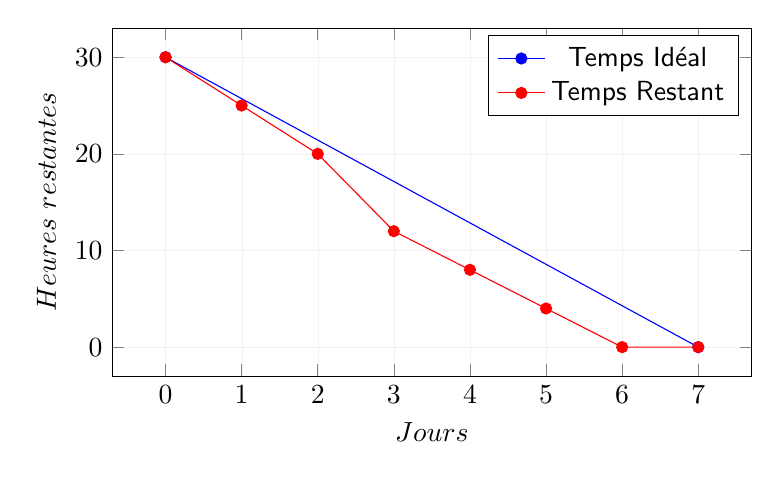
\begin{tikzpicture}[y=.2cm, x=.7cm,font=\sffamily]
\begin{axis}[
xlabel=$Jours$,
ylabel=$Heures\ restantes$,
grid=both,
grid style={line width=.1pt, draw=gray!10},
width=0.8\textwidth,
height=6cm,
%major grid style={line width=.2pt,draw=gray!50},
]
\addplot[color=blue,mark=*] coordinates {
        (0,30)
        (7, 0)
    };
    \addlegendentry{Temps Idéal}

    \addplot[mark=*,red] plot coordinates {
        (0, 30)
        (1, 25)
        (2, 20)
        (3, 12)
        (4, 8)
        (5, 4)
        (6, 0)
        (7, 0)
    };
    \addlegendentry{Temps Restant}
\end{axis}
\end{tikzpicture}
\caption{Graphique d'avancement - Itération 1}
\end{figure}


\subsection{Conclusion}
A la fin de cette itération, on avait un prototype minimale fonctionnel
dont on peut baser notre future travail.
L'approche suivi de faire le minimum des taches pendant la première itération
avait des bon effet sur les membre de notre équipe sur tout la motivation et
la solidarité.

Le tableau~\ref{tab:sprint1-evaluation} présente le pourcentage de
réalisation de nos taches de cette itération.

\begin{center}
    \begin{longtable}{| l | l |}
        \caption{Liste des tâches réalisées de la première itération}
        \label{tab:sprint1-evaluation} \\

        \hline
        \textbf{Les tâches} & \textbf{Taux de réalisation} \\ \hline
        \endhead

        \hline \multicolumn{2}{|r|}{{Continué en page suivante$\dotsc$}} \\ \hline
        \endfoot

        \hline \hline
        \endlastfoot

        \hline
Présentation et Configuration SVN & Effectué 100\% \\ \hline
Recherche sur les Services Web & Effectué 100\% \\ \hline
Implémenter service Save Position & Effectué 100\% \\ \hline
Implémenter la consommation du service Save Position & Effectué 100\% \\ \hline
Recherche sur les spécifications de la plateforme Android & Effectué 100\% \\ \hline
Création squelette de l'application mobile & Effectué 100\% \\ \hline
Implémenter service Get Last Position & Effectué 100\% \\ \hline
Rectification service Save Positon & Effectué 100\% \\ \hline
Rectification service Get Last Position & Effectué 100\% \\ \hline
Affiche Multiple marqueurs & Effectué 100\% \\ \hline
Affiche état du périphérique & Effectué 100\% \\ \hline
    \end{longtable}
\end{center}
